\documentclass[12pt]{article}

\usepackage{fullpage}

\usepackage{amsmath,amssymb,amsthm}
\usepackage{graphicx}
\usepackage{color}
\usepackage{algorithm}
\usepackage{algpseudocode}
\usepackage{hyperref}
\hypersetup{
    bookmarks=true,         % show bookmarks bar?
    unicode=false,          % non-Latin characters in Acrobat’s bookmarks
    pdftoolbar=true,        % show Acrobat’s toolbar?
    pdfmenubar=true,        % show Acrobat’s menu?
    pdffitwindow=false,     % window fit to page when opened
    pdfstartview={FitH},    % fits the width of the page to the window
    pdftitle={Computing the Riemann Constant Vector},    % title
    pdfauthor={Swierczewski, Patterson, and Deconinck},     % author
    pdfcreator={Swierczewski},   % creator of the document
    pdfkeywords={mathematics} {algebraic geometry} {riemann constant vector} {theta functions} {abel map} {jacobian},
    pdfnewwindow=true,      % links in new window
    colorlinks=false,       % false: boxed links; true: colored links
    linkcolor=red,          % color of internal links
    citecolor=green,        % color of links to bibliography
    filecolor=magenta,      % color of file links
    urlcolor=cyan           % color of external links
}
\renewcommand{\algorithmicrequire}{\textbf{Input:}\,}
\renewcommand{\algorithmicensure}{\textbf{Output:}}

%
% custom listings (code example) design
%
\usepackage{listings}
\newcounter{ipythoncounter}
\setcounter{ipythoncounter}{1}

\renewcommand{\ttdefault}{pcr}
\lstset{
  aboveskip=\bigskipamount,
  belowskip=\bigskipamount,
  basicstyle=\footnotesize\ttfamily,
  language=Python,
  numbers=left,
  stepnumber=9999,
  numberfirstline=true,
  xleftmargin=2cm,
}

\lstnewenvironment{ipythoninput}
                  {
                    \setcounter{lstnumber}{\value{ipythoncounter}}
%                    \renewcommand{\thelstnumber}
%                                 {\bf\ttfamily In [\the\value{lstnumber}]:}
                    \renewcommand{\thelstnumber}
                                 {\bf\ttfamily In [\the\value{ipythoncounter}]:}
                    \lstset{
                      frame=single,
                      frameround=tttt,
                      name=ipythoninput,
                    }
                  }
                  {
                    \addtocounter{ipythoncounter}{1}
                  }

\lstnewenvironment{ipythonoutput}
                  {
                    \addtocounter{ipythoncounter}{-1}
                    \setcounter{lstnumber}{\value{ipythoncounter}}
                    \renewcommand{\thelstnumber}
                                 {\bf\ttfamily Out[\the\value{ipythoncounter}]:}
                    \lstset{
                      name=ipythoninput
                    }
                  }
                  {
                    \addtocounter{ipythoncounter}{1}
                  }

\newtheorem{theorem}{Theorem}
\newtheorem{definition}[theorem]{Definition}

\theoremstyle{definition}
\newtheorem{example}[theorem]{Example}


\DeclareMathOperator{\ZZ}{\mathbb{Z}}
\DeclareMathOperator{\RR}{\mathbb{R}}
\DeclareMathOperator{\CC}{\mathbb{C}}
\DeclareMathOperator{\hg}{\mathfrak{h}_g}
%% \DeclareMathOperator{\dx}{dx}
%% \DeclareMathOperator{\dt}{dt}
\newcommand{\dx}{\,\mathrm{d}x}
\newcommand{\dt}{\,\mathrm{d}t}
\newcommand{\dQ}{\,\mathrm{d}Q}
\DeclareMathOperator{\DivC}{\mathcal{C}}
\DeclareMathOperator{\DivD}{\mathcal{D}}
\DeclareMathOperator{\RCV}{\boldsymbol{K}}
\DeclareMathOperator{\Abel}{\boldsymbol{A}}
\DeclareMathOperator{\HalfLattice}{\Lambda_{1/2}}

\newcommand{\thchar}[2] {\begin{bmatrix}#1\\#2\end{bmatrix}}
\newcommand{\thcharsm}[2] {\left[ \begin{smallmatrix} #1
      \\ #2 \end{smallmatrix} \right]}


\title{Computing the Riemann Constant Vector}
\author{
  \centering
  \footnotesize
  \begin{tabular}{ccc}
    % names
    Bernard Deconinck &
    Matthew Patterson &
    Chris Swierczewski \\
    % address 1
    University of Washington &
    (Matt's Address) &
    University of Washington \\
    % address 2
    Department of Applied Mathematics &
    (Matt's Address) &
    Department of Applied Mathematics \\
    % address 3
    Seattle, WA 98195-3925 &
    (Matt's Address) &
    Seattle, WA 98195-3925 \\
    % email
    \href{mailto:deconinc@uw.edu}{\tt deconinc@uw.edu} &
    \href{mailto:matt@patterson.com}{\tt matt@patterson.com} &
    \href{mailto:cswiercz@uw.edu}{\tt cswiercz@uw.edu}
  \end{tabular}
}
\date{\today}

%%%%%%%%%%%%%%%%%%%%%%%%%%%%%%%%%%%%%%%%%%%%%%%%%%%%%%%%%%%%%%%%%%%%%%%%%%%%%%%
\begin{document}
%%%%%%%%%%%%%%%%%%%%%%%%%%%%%%%%%%%%%%%%%%%%%%%%%%%%%%%%%%%%%%%%%%%%%%%%%%%%%%%

\maketitle

\begin{abstract}
The Riemann constant vector is a fundamental ingredient in the study of
Riemann surfaces and their Jacobians. It is necesasry to discuss the
Jacobi inversion problem, the study of the theta divisor, and solutions
to integrable partial differential equations.

We present a mathematical algorithm and an implementation for computing
the vector of Riemann constants on a Riemann surface given by the
desingularization and compactification of a complex plane algebraic
curve. The source code of the implementation is provided in the Python
software package {\sc abelfunctions} (\url{abelfunctions.cswiercz.info})
\end{abstract}

%%%%%%%%%%%%%%%%%%%%%%%%%%%%%%%%%%%%%%%%%%%%%%%%%%%%%%%%%%%%%%%%%%%%%%%%%%%%%%%
\section{Introduction}\label{sec:introduction}
%%%%%%%%%%%%%%%%%%%%%%%%%%%%%%%%%%%%%%%%%%%%%%%%%%%%%%%%%%%%%%%%%%%%%%%%%%%%%%%

{\it Paragraph: answer the following
\begin{itemize}
  \item What is the problem?

    Compute the Riemann constant vector for arbitrary complex plane
    curves at arbitrary places.

  \item Why is this problem important?

    RCV occurs in periodic solutions to nonlinear integrable PDEs.  A
    fundamental property of Riemann surfaces.  Primary ingredient, along
    with theta, in computing Abelian functions.

  \item What has been done for far on the problem?

    Maple implementation by Matt Patterson.  Other attempts?
    Hyperelliptic solution?  Check Fay’s thesis, Baker.

  \item What is the main contribution of the paper to the problem?

    Emphasize that it’s for a general case surface. Provide a
    step-by-step, realizable mathematical algorithm. Provide and
    describe the current implementation.

  \item Why is the contribution original?

    (literature review) Probably only done for hyperelliptic case. (?)

  \item Why is the contribution non-trivial?

    Again, general case.
\end{itemize}
}

The primary contribution of this paper is to provide an abstract
algorithm and software implementation for computing the Riemann Constant
Vector for an arbitrary Riemann surface given by the desingularization
and compactifications of a complex plane curve. An implementation of the
algorithms described in this paper is given in {\sc abelfunctions}, an
open--source Python library. The implementation details can be freely
examined in the source code at
\url{www.github.com/cswiercz/abelfunctions}. Software documentation,
including installation and use instructions, is located at
\url{abelfunctions.cswiercz.info}.




%%%%%%%%%%%%%%%%%%%%%%%%%%%%%%%%%%%%%%%%%%%%%%%%%%%%%%%%%%%%%%%%%%%%%%%%%%%%%%%
\section{Definitions and Background}\label{sec:background}
%%%%%%%%%%%%%%%%%%%%%%%%%%%%%%%%%%%%%%%%%%%%%%%%%%%%%%%%%%%%%%%%%%%%%%%%%%%%%%%

%% %------------------------------------------------------------------------------
%% \subsection{Riemann Surfaces}
%% %------------------------------------------------------------------------------

In this section the required ingredients from the theory of Riemann
surfaces are introduced. Details can be found in the standard references
\cite{FarkasKra92,Springer57} and the review paper \cite{Dubrovin81}. A
computational approach to these topics can be found in
\cite{BobenkoKlein11,DeconinckPatterson11} and
\cite{DeconinckPatterson08}.

Let $C$ be a complex plane algebraic curve $C = \{(\alpha,\beta) \in
\CC^2 : f(\alpha,\beta) = 0\}$ where $f \in \CC[x,y]$ is a polynomial
$f(x,y) = \sum_{k=0}^n \alpha_k(x) y^k$ with $\alpha_k \in \CC[x]$. Let
$X$ be the genus $g$ compact and connected Riemann surface obtained by
desingularizing and compactifying the curve $C$; i.e. $X$ is a compact,
connected, complex manifold of complex dimension one. Every compact and
connected Riemann surface can be obtained in this way
\cite{Griffiths89}.

%% The first homology group $H_1(X,\ZZ)$ of $X$ is the collection of all
%% cycles on $X$ modulo homologous transformations. $H_1(X,\ZZ)$ has a
%% canonical basis of cycles $\{a_1,\ldots,a_g,b_1,\ldots,b_g\}$. The space
%% of holomorphic 1-forms $\Gamma(X,\Omega_X^1)$ on $X$ is the collection
%% of all 1-forms $\omega \in \Omega_X^1$ such that for each local
%% coordinate $z_\alpha : U_\alpha \subset X \to \CC$,
%% \begin{equation}
%%   \omega \big|_{U_\alpha}  = h_\alpha(z_\alpha) dz_\alpha
%% \end{equation}
%% where $h_\alpha : U_\alpha \to \CC$ is a holomorphic
%% function. $\Gamma(X,\Omega_X^1)$ has a basis of holomorphic one-forms
%% $\{\omega_1, \ldots, \omega_g\}$.
Given $X$ of genus $g$ we choose a canonical basis of cycles
$\{a_1,\ldots,a_g,b_1,\ldots,b_g\}$ for the first homology group as well
as a normalized basis of Abelian differentials of the first kind
$\{\omega_1, \ldots, \omega_g\}$. We define the Jacobian $J(X)$ of $X$
using these two ingredients. Construct the {\it period matrix} $\tau =
[I \; \; \Omega] \in \CC^{g \times 2g}$ of $X$ where
\begin{equation} \label{eqn:periodmatrix}
  \oint_{a_j} \omega_i = \delta_{ij}, \qquad
  \oint_{b_j} \omega_i = \Omega_{ij}.
\end{equation}
The matrix $\Omega \in \CC^{g \times g}$ is a {\it Riemann matrix}: a
symmetric complex $g \times g$ matrix with positive definite imaginary
part. The Jacobian is given by the quotient space $J(X) = \CC^g /
\Lambda$ where $\Lambda = \ZZ^g + \Omega \ZZ^g$ is a lattice in
$\CC^g$.

An algorithm for computing a canonical basis of cycles, a basis of
Abelian differentials of the first kind, and Riemann matrices is
described in \cite{DeconinckPatterson08}. The basis of differentials
$\{\tilde{\omega}_1, \ldots, \tilde{\omega}_g\}$ returned by this
algorithm is not necessarily normalized. If a normalized basis is
desired one can be determined by computing the period matirx $\tau = [A
  \;\; B]$ defined by
\begin{equation} \label{eqn:periodmatrixnotnormal}
  \oint_{a_j} \tilde{\omega}_i = A_{ij}, \qquad
  \oint_{b_j} \tilde{\omega}_i = B_{ij}.
\end{equation}
The associated Riemann matrix is constructed by setting $\Omega =
A^{-1}B$ and normalized basis of Abelian differentials by determining
$\boldsymbol{\omega} = A^{-1}\tilde{\boldsymbol{\omega}}$ where
$\tilde{\boldsymbol{\omega}} = [\tilde{\omega}_1, \ldots,
  \tilde{\omega}_g]^T$.


\begin{example} \label{ex:riemannsurface} %%%%%%%%%%%%%%%%%%%%%%%%%%%%%%%%%%%%%
Let $X$ be the Riemann surface obtained from the curve
\begin{equation}
  C: f(x,y) = x^2y^3 - x^4 + 1 = 0.
\end{equation}
We will use this Riemann surface as an example throughout this paper. We
first compute a basis, not necessarily normalized, for the space of
Abelian differentials of the first kind.
\begin{ipythoninput}
from abelfunctions import *
from sympy.abc import x,y

f = x**2*y**3 - x**4 + 1
X = RiemannSurface(f,x,y)    # the primary object in abelfunctions
g = X.genus()

omega = X.holomorphic_differentials()
print 'differentials:', omega
print 'genus:', g
\end{ipythoninput}
\begin{ipythonoutput}
differentials: [1/(3*x**2*y**2), 1/(3*x*y**2), 1/(3*x*y), 1/(3*y**2)]
genus: 4
\end{ipythonoutput}
Next, we compute a canonical basis of cycles on $X$. We plot the
projection of the cycle $a_1$ in the complex $x$- and $y$-planes.
\begin{ipythoninput}
a = X.a_cycles()
b = X.b_cycles()

# use 256 points to plot the x- and y-parts of the path
a[0].plot_x(256, 'blue', linewidth=2)
a[0].plot_y(256, 'green', linewidth=2)
\end{ipythoninput}
\vspace{-12pt}
\begin{ipythonoutput}
\end{ipythonoutput}
\hspace{2pt} {\footnotesize\bf\ttfamily Out[2]:}

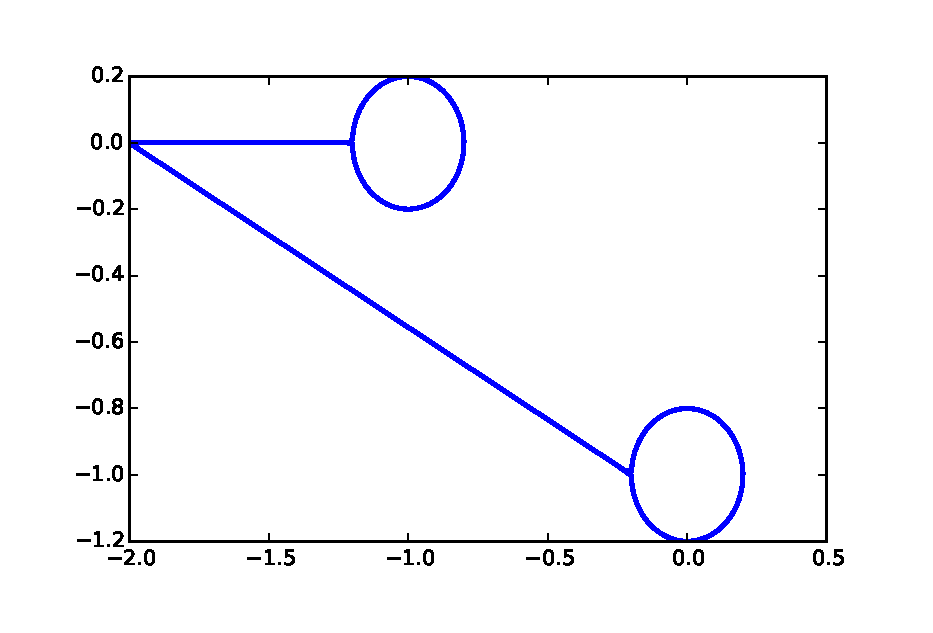
\includegraphics[width=0.45\textwidth]{a1x.eps}
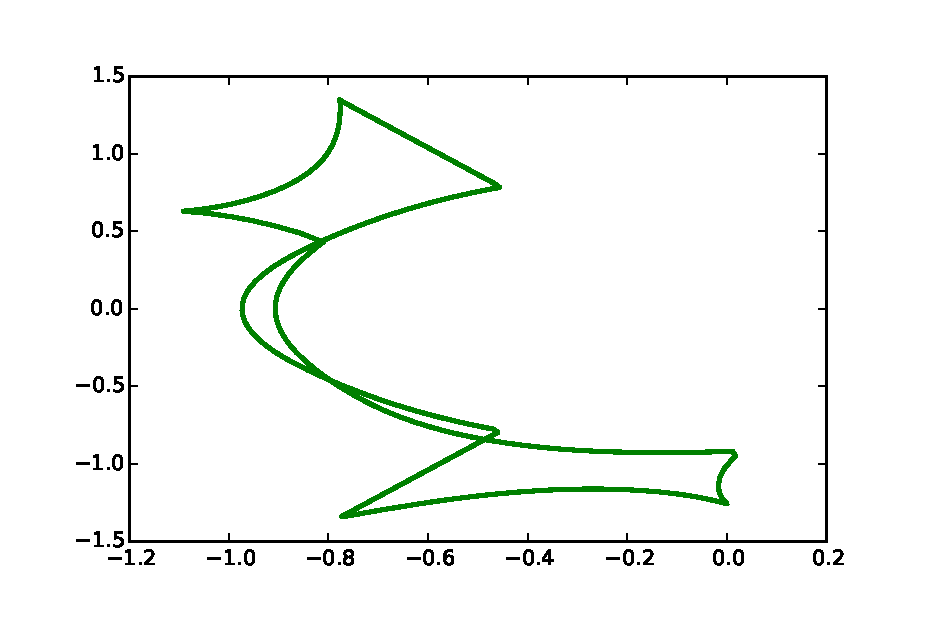
\includegraphics[width=0.45\textwidth]{a1y.eps}

These holomorphic differentials are not normalized, as indicated by the
period matrix.
\begin{ipythoninput}
tau = X.period_matrix()
A = tau[:,:g]
B = tau[:,g:]

# only print the first two significant digits, for clarity
import numpy
numpy.set_printoptions(precision=2,suppress=True)

print A
print
print B
\end{ipythoninput}
\begin{ipythonoutput}
[[ 0.28+1.04j  0.28-0.48j -1.81+1.04j  0.00-0.j  ]
 [ 0.66-1.15j  0.66+0.38j -0.66-1.15j -0.00+1.53j]
 [-0.83+0.48j -0.83+0.48j  0.83-1.45j  0.00+1.93j]
 [-1.04+0.28j -1.04+1.81j -0.48+0.28j  0.00+0.j  ]]

[[-0.28+0.48j  0.28-1.04j  0.00-2.09j  0.76-1.32j]
 [ 0.66+0.38j -0.66+0.38j  0.00-0.76j  0.00-1.53j]
 [-0.83+0.48j  0.83-1.45j  0.00-0.96j -1.67-0.96j]
 [ 1.04-1.81j -1.04-0.28j -0.00-0.56j  0.76-1.32j]]
\end{ipythonoutput}
\end{example}




%------------------------------------------------------------------------------
\subsection{Places and Divisors}
%------------------------------------------------------------------------------


\begin{definition}\label{def:puiseux}
Given a place $P \in X$ a local representation of the Riemann surface
centered at $P$ is given using a Puiseux series
\begin{align} \label{eqn:puiseux}
  P =
  \begin{cases}
    x_P(t) = \alpha + \lambda t^e, \\
    y_P(t) = \sum_{k=0}^\infty \beta_k t^{n_k},
  \end{cases}
\end{align}
where $\alpha, \lambda, \beta_k \in \CC$, and $e, n_k \in \ZZ$.
\end{definition}
\noindent Places lie ``above'' the curve $C$ in the sense that
evaluating $P = (x_P(t), y_P(t))$ at $t=0$ maps the place $P$ onto a
point $(\alpha,\beta)$ of the curve.

Let $R(f,\partial_y f)(x)$ be the resultant of $f(x,y)$ and $\partial_y
f(x,y)$ with respect to $y$ \cite{Griffiths89}. The roots $\alpha \in
\CC$ of $R$ correspond to the {\it discriminant points} of $C$, which
consist of the branch points and singular points of the curve. A place
is called {\it discriminant} if it lies above a discriminant point of
$C$. Otherwise, it is {\it regular}. An algorithm for computing Puiseux
series expansions is found in \cite{Duval89} and
\cite{PoteauxRybowicz08}.


\begin{example} \label{ex:places} %%%%%%%%%%%%%%%%%%%%%%%%%%%%%%%%%%%%%%%%%%%%%
Continuing from Example \ref{ex:riemannsurface}, there is one place on
$X$ lying above the discriminant point $x=0$
\begin{equation}
  P =
  \begin{cases}
    x_{P}(t) &= -t^3 \\
    y_{P}(t) &= -t^{-2} + O\left( t^2 \right).
  \end{cases}
\end{equation}
and there are three regular places lying above $x=2$
\begin{equation}
  P_1 =
  \begin{cases}
    x_{P_1}(t) &= 2 + t \\
    y_{P_1}(t) &= [XXX],
  \end{cases} \quad
  P_2 =
  \begin{cases}
    x_{P_2}(t) &= 2 + t \\
    y_{P_2}(t) &= [XXX],
  \end{cases} \quad
  P_3 =
  \begin{cases}
    x_{P_3}(t) &= 2 + t \\
    y_{P_3}(t) &= [XXX].
  \end{cases}
\end{equation}
We confirm the form of these places computationally:
\begin{ipythoninput}
places_above_zero = X(0)
print places_above_zero
\end{ipythoninput}
\begin{ipythonoutput}
[(-t**3, -1/t**2 + O(t**2))]
\end{ipythonoutput}
\begin{ipythoninput}
places_above_two = X(2)
for P in places_above_two:
    print P
\end{ipythoninput}
\begin{ipythonoutput}
(t + 2, XXX)
(t + 2, XXX)
(t + 2, XXX)
\end{ipythonoutput}

\end{example}

Related to places is the notion of a divisor.
\begin{definition} \label{def:divisor}
A divisor $\DivD$ on the Riemann surface $X$ is a finite formal linear
combination of places $P_i$ with multiplicities $n_i$:
\begin{equation}
\DivD = \sum_i n_i P_i.
\end{equation}
The sum
\begin{equation}
\deg \DivD = \sum_i n_i
\end{equation}
is called the degree of $\DivD$.
\end{definition}
The set of all divisors forms an Abelian group $\text{Div}(X)$ under
addition. A divisor with all $n_i \geq 0$ is called {\it positive} or
{\it effective}. A {\it valuation divisor}, important for the
calculation of the Riemann constant vector, is obtained by examining the
root and pole structure of a meromorphic one-form on $X$.
\begin{definition} \label{def:valuationdivisor}
Let $\Omega_X^1$ denote the set of meromorphic one-forms on $X$ and let
$\nu \in \Omega_X^1$ have $m$ zeros of multiplicity $p_j$ at the places
$P_j$ and $n$ poles of multiplicity $q_j$ at the places $Q_j$. Then
\begin{equation} \label{eqn: valuation divisor}
  (\nu)_\text{val} = \sum_{i=1}^m p_iP_i - \sum_{j=1}^n q_jQ_j
\end{equation}
is called the valuation divisor of $\nu$. A divisor $\DivC \in
\text{Div}(X)$ is called {\it canonical} if $\DivC = (\nu)_\text{val}$
for some $\nu \in \Omega_X^1$.
\end{definition}
All canonical divisors have the same degree and, by the Riemann--Roch
theorem, this degree is $\deg \DivC = 2g - 2$ \cite{Springer57}. Note
that every Abelian differential of the first kind is trivially
meromorphic, since it is a holomorphic one-form, and its valuation
divisor has $q_j = 0$ for all $j$. Consequently, every such differential
has exactly $2g-2$ zeros including multiplicities.


\begin{example} \label{ex:divisors} %%%%%%%%%%%%%%%%%%%%%%%%%%%%%%%%%%%%%%%%%%%
We use the places computed in Example \ref{ex:places} to construct
divisors on the Riemann surface $X$.
\begin{ipythoninput}
P = places_above_zero[0]
Q = places_above_two[0]
D = 3*P + Q
print D
print D.degree()
\end{ipythoninput}
\begin{ipythonoutput}
[XXX]
\end{ipythonoutput}
\end{example}


%------------------------------------------------------------------------------
\subsection{The Abel Map}
%------------------------------------------------------------------------------

\begin{definition}\label{def:abelmap}
  Let $P \in X$ be a fixed place. The Abel Map $\boldsymbol{A} : X \to
  J(X)$ is defined
  \begin{equation} \label{eqn:abel1}
    \boldsymbol{A}(P,Q) = \big( A_1(P,Q), \ldots, A_g(P,Q) \big),
  \end{equation}
  where
  \begin{equation} \label{eqn:abel2}
    A_j(P,Q) = \int_P^Q \omega_j,
  \end{equation}
  and the path chosen from $P$ to $Q$ is the same for each $A_j$. The
  Abel map is written in vector form as
  \begin{equation} \label{eqn:abel-vector}
    \boldsymbol{A}(P,Q) = \int_P^Q \boldsymbol{\omega}.
  \end{equation}
\end{definition}
The definition of the Abel map can be extended to divisors: let $\DivD =
\sum_i n_i P_i$. We define
\begin{equation} \label{eqn:abel-divisors}
  \boldsymbol{A}(P,\DivD) = \sum_i n_i \boldsymbol{A}(P,P_i).
\end{equation}
The Abel Map is independent of the path $\gamma$ from $P$ to $Q$ chosen
on $X$ for if $\gamma$ and $\eta$ are two such paths then their
difference is a linear combination of homology basis cycles. The
integral of $\boldsymbol{\omega}$ along this closed path is a lattice
element and therefore is congruent to zero in $J(X)$.

An algorithm for computing the Abel map is described in
\cite{DeconinckPatterson11} on which the implementation in {\sc
  abelfunctions} is based.

\begin{example}
{\sc abelfunctions} selects a ``base place'' $P_0$ from which to
construct all paths on $X$. When given a single argument, the function
{\tt Abel()} returns $\Abel(P_0,P)$.
\begin{ipythoninput}
z1 = Abel(P)      # Abel map from P0 to P
z2 = Abel(Q)      # Abel map from P0 to Q
z3 = Abel(P,Q)    # Abel map from P to Q
print z1
print z2
print z3
\end{ipythoninput}
\begin{ipythonoutput}
[XXX]
[XXX]
[XXX]
\end{ipythonoutput}
The Abel map accepts divisors as well.
\begin{ipythoninput}
w = Abel(D)    # D = 3P + Q

# reduce 3*z1+z2 modulo the Jacobian lattice
J = X.Jacobian()
z = J(3*z1 + z2)

# confirm that the two results are identical
from scipy.linalg import norm
print norm(w-z)
\end{ipythoninput}
\begin{ipythonoutput}
[XXX]
\end{ipythonoutput}

\end{example}



%------------------------------------------------------------------------------
\subsection{The Riemann Constant Vector}
%------------------------------------------------------------------------------

\begin{definition} \label{def:rcv}
Let $X$ be a genus $g$ Riemann surface with associated Riemann matrix
$\Omega$. The Riemann constant vector $\RCV : X \to J(X)$ is defined as
\begin{equation} \label{eqn:rcv1}
  \RCV(P) = \big( K_1(P), \ldots, K_g(P) \big),
\end{equation}
where
\begin{equation} \label{eqn:rcv2}
  K_j(P) = \frac{1 + \Omega_{jj}}{2} - \sum_{k \neq j}^g
           \oint_{a_k} \omega_k(Q) A_j(P,Q).
\end{equation}
\end{definition}
Once we know the value of $\RCV(P_0)$ the value of $\RCV(P)$ is
determined using only a shift by the Abel map:
\begin{theorem} \label{thm:RCVshift}
  Let $P_0,P$ be places on a genus $g$ Riemann surface $X$. Then
  \begin{equation} \label{eqn:RCVshift}
    \RCV(P) = \RCV(P_0) + (g-1)\Abel(P_0,P).
  \end{equation}
\end{theorem}
\begin{proof}
Let $Q$ be an arbitrary place on $X$. By the definition of the Abel map,
$\Abel(P,Q) = \Abel(P,P_0) + \Abel(P_0,Q)$. Using this identity in the
definition of the RCV we obtain
\begin{align} \label{eqn:RCVshift1}
  K_j(P)
  &=
  \frac{1 + \Omega_{jj}}{2}
  -
  \sum_{k \neq j}^g
  \oint_{a_k} \omega_k(Q) A_j(P,Q) \dQ  \notag \\
  &=
  \frac{1 + \Omega_{jj}}{2}
  -
  \sum_{k \neq j}^g
  \oint_{a_k} \omega_k(Q) \Big( A_j(P,P_0) + A_j(P_0,Q) \Big) \dQ  \notag \\
  &=
  \frac{1 + \Omega_{jj}}{2}
  -
  \sum_{k \neq j}^g
  \oint_{a_k} \omega_k(Q) A_j(P,P_0) \dQ
  -
  \sum_{k \neq j}^g
  \oint_{a_k} \omega_k(Q) A_j(P_0,Q) \dQ.
\end{align}
The $j$th-component of the Abel map appearing in the first sum has no
dependence on the variable of integration $Q$ nor on the summation index
$k$. Therefore,
\begin{align} \label{eqn:RCVshift2}
  K_j(P)
  &=
  \frac{1 + \Omega_{jj}}{2}
  -
  \sum_{k \neq j}^g
  A_j(P,P_0)
  \oint_{a_k} \omega_k(Q) \dQ
  -
  \sum_{k \neq j}^g
  \oint_{a_k} \omega_k(Q) A_j(P_0,Q) \dQ \notag \\
  &=
  \frac{1 + \Omega_{jj}}{2}
  -
  (g-1) A_j(P,P_0)
  -
  \sum_{k \neq j}^g
  \oint_{a_k} \omega_k(Q) A_j(P_0,Q) \dQ \notag \\
  &=
  K_j(P_0) + (g-1)A_j(P_0,P).
\end{align}
\end{proof}
The primary computational benefit to using the result of Theorem
\ref{thm:RCVshift} is that most of the work in evaluating $\RCV$ comes
from evaluating it at a fixed place $P_0$. Once this is done, we only
need the Abel map to determine $\RCV$ for all other places $P \in X$. In
{\sc abelfunctions} a fixed place of the Riemann surface is
automatically chosen.

The inspiration behind the algorithm for computing the RCV described in
the following section comes from the following two theorems. Theorem
\ref{thm:rcvequiv} characterizes a certain class of divisors in terms of
the RCV, a proof of which is found in \cite{FarkasKra92}.
\begin{theorem} \label{thm:rcvequiv}
  Let $\DivC$ be a divisor on a genus $g$ Riemann surface $X$ of degree
  $2g - 2$. Then $\DivC$ is a canonical divisor if and only if
  \begin{equation} \label{eqn:rcvequiv}
    2\RCV(P) \equiv -\Abel(P,\DivC).
  \end{equation}
\end{theorem}
\noindent Theorem \ref{thm:thetadivisor} establishes a connection
between the Riemann theta function and the RCV, a proof of which is also
found in \cite{FarkasKra92}.
\begin{definition} \label{def:riemanntheta}
  The Riemann theta function $\theta: J(X) \times \hg \to \CC$ is
  defined by
  \begin{equation} \label{eqn:riemanntheta}
    \theta(z,\Omega)
    =
    \sum_{n \in \ZZ^g}
    e^{2 \pi i \left( \tfrac{1}{2} n \cdot \Omega n + n \cdot z \right)}.
  \end{equation}
  This function converges absolutely and uniformly on compact sets in
  $J(X) \times \hg$ where $\hg$ is the space of all Riemann matrices.
\end{definition}

\begin{theorem} \label{thm:thetadivisor}
  Let $\Omega$ be the Riemann matrix associated with the Riemann surface
  $X$ and $P_0 \in X$ an arbitrary place. Then a vector $\boldsymbol{W}
  \in J(X)$ satisfies
  \begin{equation} \label{eqn:thetadivisor1}
    \theta(\boldsymbol{W}, \Omega) = 0
  \end{equation}
  if and only if there exists a divisor $\DivD = P_1 + \cdots P_{g-1}$
  such that
  \begin{equation} \label{eqn:thetadivisor2}
    \boldsymbol{W} = \boldsymbol{A}(P_0, \DivD) + \boldsymbol{K}(P_0).
  \end{equation}
\end{theorem}
Note that $\DivD$ may contain a place of multiplicity greater than
one. The primary requirement of $\DivD$ is that it is of degree $g-1$
and is effective. The set $\Theta := \{ \boldsymbol{W} \in J(X) :
\theta(\boldsymbol{W},\Omega) = 0\}$ is known as the {\it theta divisor}
of the Riemann surface $X$. It is a $(g-1)$ complex--dimensional
subvariety of $J(X)$. Theorem \ref{thm:thetadivisor} states that $\Theta
= \Abel\left(P_0,SX^{g-1}\right) + \boldsymbol{K}(P_0)$ where $SX^{g-1}$
is the $(g-1)$--fold symmetric product of the Riemann surface.




%%%%%%%%%%%%%%%%%%%%%%%%%%%%%%%%%%%%%%%%%%%%%%%%%%%%%%%%%%%%%%%%%%%%%%%%%%%%%%%
\section{Computing the Riemann Constant Vector}
%%%%%%%%%%%%%%%%%%%%%%%%%%%%%%%%%%%%%%%%%%%%%%%%%%%%%%%%%%%%%%%%%%%%%%%%%%%%%%%





In this section we present an algorithm for computing the Riemann
constant vector as well as a demonstration of its implementation in {\sc
  abelfunctions}. We first present an overview of and motivation behind
the algorithm and describe the two primary components of the algorithm
later in this section.

Theorem \ref{thm:rcvequiv} suggests an approach to computing the RCV
provided we can compute a canonical divisor of the Riemann
surface. However, even with such a divisor the theorem only makes a
statement about the value of $2\RCV(P_0)$. That is, one would like to
say
\begin{equation}
\RCV(P_0) \equiv - \tfrac{1}{2} \Abel(P_0,\DivC)
\end{equation}
but division is not unique modulo the lattice $\Lambda$. In general,
there are $2^{2g}$ {\it half-lattice vectors} $\boldsymbol{h} \in
\tfrac{1}{2}\Lambda$ such that $\RCV(P_0) \equiv \boldsymbol{h} -
\tfrac{1}{2}\Abel(P_0,\DivC)$. Therefore, a second objective is to find
an appropriate half-lattice vector.

\begin{algorithm}[H]
\caption{\tt riemann\_constant\_vector}
\label{alg:rcv}
\begin{algorithmic}[1]
  \Require Riemann surface $X$ given by the desingularization and
  compactification of complex plane algebraic curve $C : f(x,y) = 0$

  \Require place $P \in X$

  \Ensure Riemann constant vector $\RCV(P)$

  \State compute the Riemann matrix $\Omega$

  \State $\DivC \gets$ \verb=canonical_divisor()=
  \Comment{Algorithm \ref{alg:canonical}}

  \State $\boldsymbol{h} \gets$ \verb=half_lattice_vector()=
  \Comment{Algorithm \ref{alg:half-lattice-vector}}

  \State $\RCV_0 \gets \boldsymbol{h} - \tfrac{1}{2}\Abel(P_0,\DivC)
  \bmod{\Lambda}$

  \For{$j = 1,\ldots,g$}

      \State $K_j \gets \tfrac{1}{2}(1+\Omega_{jj}) + (g-1)A_j(P_0,P) -
      (\RCV_0)_j$

  \EndFor

  \State \Return $\RCV = (K_1, \ldots, K_g)$
\end{algorithmic}
\end{algorithm}

The rest of this section presents in detail the subroutines
\verb=canconical_divisor= and \verb=half_lattice_vector= which provide
the necessary remaining ingredients for the above algorithm.



%------------------------------------------------------------------------------
\subsection{Computing a Canonical Divisor}\label{sec:canonical}
%------------------------------------------------------------------------------



Determining the zeros and poles of a meromorphic one-form
\begin{equation} \label{eqn:meromorphic-one-form}
\nu = \frac{p(x,y)}{q(x,y)}\dx
\end{equation}
is not as straightforward as finding the roots of the polynomials $p$
and $q$. One challenge comes from analyzing the local behavior of
$\dx$. Furthermore, it may occur that the numerator and denominator have
the same order of vanishing at some place $P \in X$ in which case $P$ is
neither a root nor pole of $\nu$.

Let $P \in X$ be a place with Puiseux series representation $(x_P(t),
y_P(t))$ where $t$ is a local parameter as given in Definition
\ref{def:puiseux}. A necessary condition for $P$ to be a root or pole of
$\nu$ is that
\begin{equation}
  p\big(x_P(t), y_P(t)\big) \Big|_{t=0} \! = 0,
  \qquad
  q\big(x_P(t), y_P(t)\big) \Big|_{t=0} \! = 0,
  \qquad \text{or} \qquad
  \frac{dx_P}{dt}\big(0\big) = 0.
\end{equation}
In particular, given some $P \in X$ to determine if $P \in
(\nu)_\text{val}$ we substitute the Puiseux series representation into
$\nu$ and expand as a Laurent series in $t$:
\begin{align} \label{eqn:localization}
\nu \Big|_P
&=
\frac{p\big(x_P(t),y_P(t)\big)}{q\big(x_P(t),y_P(t)\big)} \dx_P(t) \notag \\
&=
\frac{p(t)}{q(t)} x_P'(t) \dt \notag \\
&=
\Big( c t^{\text{val}(\nu,P)} + \cdots \Big) \dt
\end{align}
where $\text{val}(\nu,P)$ is the leading order behavior of $\nu$ at
$P$. This gives us a test for determining if $P$ is a member of the set
of places appearing in $(\nu)_\text{val}$: if $\text{val}(\nu,P) < 0$
then $P$ is a pole, if $\text{val}(\nu,P) > 0$ then $P$ is a zero,
otherwise $P$ does not appear in the valuation divisor of $\nu$. The
multiplicity of the zero or pole is equal to $|\text{val}(\nu,P)|$.

With the above membership test what remains is to construct a set of
places $\mathcal{P}_\nu$ guaranteed to contain the places appearing in
$(\nu)_\text{val}$. We obtain the valuation divisor by applying the
membership test to each $P \in \mathcal{P}_\nu$. Consider the resultant
$R(f,p)(x)$ of $f$ and $p$ with respect to $y$. By definition, the roots
of $R$ are the points $\alpha \in \CC$ such that
\begin{equation}
f(\alpha,y) = 0 \quad \text{and} \quad p(\alpha, y) = 0
\end{equation}
have simultaneous solutions. Therefore, for a place $P$ to be a zero of
$p$ it must be the case that the $x$-projection of $P$, $x_P(0)$, is a
root of the resultant $R$. Similarly, for $P$ to be a zero of $q$ its
$x$-projection $x_P(0)$ must be a root of the resultant $R(f,q)(x)$. We
also need to include the places $P$ which cause $\dx$ to vanish. This
occurs when $\dx_P(0) = x'_P(0) = 0$. That is, when $P$ lies above a
branch point of $f$.

Define the sets
\begin{align}
\mathcal{X}_\nu^{(1)} &=
\left\{
\alpha \in \CC \; | \; R(f,p)(\alpha) = 0
\right\}, \notag \\
\mathcal{X}_\nu^{(2)} &=
\left\{
\alpha \in \CC \; | \; R(f,q)(\alpha) = 0
\right\}, \quad \text{and} \notag \\
\mathcal{X}_\nu^{(3)} &= \left\{ \alpha \in \CC \; | \; \alpha \text{ is
  a branch point of $f$} \right\}.
\end{align}
Since the representation of the one-form in Equation
\eqref{eqn:meromorphic-one-form} only captures its affine behavior it is
necessary to examine its behavior at all places lying above
$x=\infty$. Define
\begin{equation}
\mathcal{X}_\nu
=
\mathcal{X}_\nu^{(1)} \cup
\mathcal{X}_\nu^{(2)} \cup
\mathcal{X}_\nu^{(3)} \cup
\{ \infty \}.
\end{equation}
This consists of all $x$-points above which there may be a place $P$
where $\nu$ vanishes. That is, the only places we need to check are
those with $x$-projections in $\mathcal{X}_\nu$. Therefore, the set
\begin{equation}
\mathcal{P}_\nu =
\left\{ P \in X \; | \; x_P(0) \in \mathcal{X}_\nu
\right\}.
\end{equation}
is guaranteed to contain the places appearing in $(\nu)_\text{val}$. The
Puiseux algorithm is well-designed to compute this set.

This procedure is simplified when computing the valuation divisor of an
Abelian differential of the first kind. Recall that every such
differential is trivially a meromorphic one-form and therefore can be
used to compute a canonical divisor. We could use one of the normalized
basis elements $\{\omega_1, \ldots, \omega_g\}$ to obtain a canonical
divisor on $X$ but it is preferred to use the non-normalized
differentials $\{\tilde{\omega}_1, \ldots, \tilde{\omega}_g\}$ returned
by {\sc abelfunctions}. This is done for several performance-related
reasons.
\begin{itemize}
\item We already compute these differentials for the purposes of
  determining the period matrix of $X$ as well as in defining the Abel
  map.
\item Fewer resolvent sets need to be determined. The denominator of
  every Abelian differential of the first kind is $\partial_y f(x,y)$
  \cite{Noether83,Brieskorn86} so one can compute the resolvent set of
  $f$ with $\partial_y f$ once and use the results for each holomorphic
  one-form. This particular resolvent set consists of the discriminant
  points of $f$ and is already used in the period matrix calculations.
\item The set of $P$ such that $x_P(0)$ is a branch point of $f$ is
  contained in the set of discriminant points of $f$. Therefore, the set
  $\mathcal{X}_{\tilde{\omega}}^{(3)}$ is a redundant calculation and is
  omitted.
\item In general, the valuation divisors of holomorphic one-forms
  consist of fewer distinct places. The degree of every canonical
  divisor is $2g-2$. Therefore, there must always be $2g-2$ more zeros
  than poles, counting multiplicities. Thus, using Abelian differentials
  of the first kind minimizes the total number of place to check.
\item Algorithm \ref{alg:canonical} iteratively checks each $P \in
  \mathcal{P}_{\tilde{\omega}}$ for membership in the set of places in
  $\DivC = (\tilde{\omega})_\text{val}$. By using these differentials we
  can terminate this proceedure the moment $\deg \DivC$ reaches $2g-2$
  for each $P\in\mathcal{P}{\tilde{\omega}}$ contributes a non-negative
  amount to the degree. For this reason, we distinguish between the set
  of $\mathcal{X}_\omega$ and corresponding places $\mathcal{P}_\omega$
  in order to avoid unnecessarily computing Puiseux series expansions.
\end{itemize}

An algorithm for computing the valuation divisor of a holomorphic
one-form is given below.
\begin{algorithm}[H]
\caption{{\tt canonical\_divisor} - canonical divisor of a Riemann surface}
\label{alg:canonical}
\begin{algorithmic}[1]
  \Require Riemann surface $X$ given by the desingularization and
  compactification of complex plane curve $C : f(x,y) = 0$

  \Require an Abelian differential of the first kind $\tilde{\omega} =
  p(x,y) / \partial_y f(x,y) \dx$ on $X$

  \Ensure canonical divisor $\DivC = (\tilde{\omega})_\text{val}$

  \State $\DivC \gets$ zero divisor

  \State $\mathcal{X}_{\tilde{\omega}}^{(1)} \gets$ roots of resolvent
  $R(f,p)(x) = 0$

  \State $\mathcal{X}_{\tilde{\omega}}^{(2)} \gets$ discriminant points of $f$

  \State $\mathcal{X}_{\tilde{\omega}} \gets
  \mathcal{X}_{\tilde{\omega}}^{(1)} \cup
  \mathcal{X}_{\tilde{\omega}}^{(2)} \cup \{ \infty \}$

  \For{$\alpha \in \mathcal{X}_{\tilde{\omega}}$}

  \State $\mathcal{P}_{\tilde{\omega}}^\alpha \gets \left\{ P \in X \; |
  \; x_P(0) = \alpha \right\}$

  \For{$P \in \mathcal{P}_{\tilde{\omega}}^\alpha$}

  \State $n \gets \text{val}\left(\tilde{\omega},P\right)$

  \State $\DivC \gets \DivC + \,n P$

  \If{$\deg \DivC = 2g - 2$}
  \State \Return $\DivC$
  \EndIf

  \EndFor

  \EndFor

  \State {\bf raise error}(``Not enough places found.'')

\end{algorithmic}
\end{algorithm}
Some notes about the algorithm:
\begin{itemize}
\item Only the leading order behavior of the Puiseux series of each
  place $P \in \mathcal{P}_\omega^\alpha$ determining
  $\text{val}(\tilde{\omega},P)$ is needed implying that computing only
  the ``singular part'' of these expansions using the method of Duval is
  sufficient \cite{Duval89}.
\item Since any Abelian differential of the first kind is sufficient for
  computing a canonical divisor we can choose the basis element
  $\tilde{\omega}_i$ with lowest total degree numerator $p=p(x,y)$ to
  reduce the number of places to check and amount of symbolic arithmetic
  to perform.
\item Algorithm \ref{alg:canonical} terminate once the target degree is
  met and will spend no further effort computing places and
  valuations. A significant gain in efficiency is observed when
  $\mathcal{X}_{\tilde{\omega}}$ is ordered such that places over $x,y
  \in \{0,\infty\}$ are checked first since the numerators of
  $\tilde{\omega}_i$ tend to be monomial. For testing purposes, the
  algorithm can be modified to verify that $\text{val}(\tilde{\omega},P)
  = 0$ for all remaining $P \in \mathcal{P}_{\tilde{\omega}}$.
\item If the main loop in Algorithm \ref{alg:canonical} terminates
  before the requisite degree is achieved then an error is
  reported. This is included as a sanity check for the algorithm. An
  additional test is to verify that $\deg (\tilde{\omega}_i)_\text{val}
  = 2g-2$ for all $\tilde{\omega}_i$ basis elements however because it
  is an expensive calculation it is not performed by default and is
  instead relegated to the {\sc abelfunctions} test suite.
\end{itemize}

\begin{example} \label{ex:canonical} %%%%%%%%%%%%%%%%%%%%%%%%%%%%%%%%%%%%%%%%%%
We compute a canonical divisor using the differentials from Example
\ref{ex:riemannsurface}.
\begin{ipythoninput}
C0 = omega[0].valuation_divisor()
for multiplicity, place in C0:
    print multiplicity
    print place
    print

print 'Degree:', C0.degree
\end{ipythoninput}
\begin{ipythonoutput}
[XXX]
\end{ipythonoutput}
\begin{ipythoninput}
C1 = omega[1].valuation_divisor()
for multiplicity, place in C1:
    print multiplicity
    print place
    print

print 'Degree:', C1.degree
\end{ipythoninput}
\begin{ipythonoutput}
[XXX]
\end{ipythonoutput}
\end{example}




%------------------------------------------------------------------------------
\subsection{Computing a Half-Lattice Vector}
%------------------------------------------------------------------------------


Now that we have a canonical divisor $\DivC$ it remains to determine
$\RCV(P_0)$ knowing that $2\RCV(P_0) \equiv - \Abel(P_0,\DivC)
\bmod{\Lambda}$. For now, consider $\RCV(P_0)$ and $\Abel(P_0,\DivC)$ to
be vectors in $\CC^g$ and set $\RCV_0 := \RCV(P_0)$ and $\Abel_0^{\DivC}
:= \Abel(P_0,\DivC)$, for notational convenience. In $\CC^g$ we have
\begin{equation}
2\RCV_0 + \Abel_0^{\DivC} = \boldsymbol{\lambda}
\end{equation}
where $\boldsymbol{\lambda} \in \CC^g$ is unknown and
$\boldsymbol{\lambda} \equiv 0 \bmod{\Lambda}$, i.e. the vector
$\boldsymbol{\lambda}$ is one of the $2^{2g}$ lattice vectors lying in
the fundamental region of $\Lambda$. Division by two is now legal:
setting $\boldsymbol{h} = \boldsymbol{\lambda}/2$ yields
\begin{equation}
\RCV_0 = \boldsymbol{h} - \tfrac{1}{2} \Abel(P_0,\DivC).
\end{equation}
Reducing this expression modulo $\Lambda$ gives the corresponding
equivalence in $J(X)$
\begin{equation}
\RCV_0 \equiv \boldsymbol{h} - \tfrac{1}{2} \Abel(P_0,\DivC)
\bmod{\Lambda}
\end{equation}
where the lattice vector $\boldsymbol{h}$ is unknown.

To determine which of the $2^{2g}$ half-lattice vectors
$\boldsymbol{h}_j, j = 1, \ldots, 2^{2g}$ is the correct half-lattice
vector we use Theorem \ref{thm:thetadivisor}. The Theorem requires a
degree $g-1$ effective divisor. Consider the divisor
\begin{equation} \label{eqn:simple-effective-divisor}
  \DivD = (g-1)P_0
\end{equation}
where $P_0 \in X$ is the fixed place [XXX]. Then
\begin{align*}
  \theta\big(\Abel(P_0,\DivD) + \RCV(P_0)\big)
  &=
  \theta\bigg(\Abel\big(P_0,(g-1)P_0\big) + \RCV(P_0)\bigg) \notag \\
  &=
  \theta\big(\boldsymbol{0} + \RCV(P_0)\big) \notag \\
  &=
  \theta\big(\RCV(P_0)\big) = 0.
\end{align*}
Therefore, it is necessary that
\begin{equation}
  \theta\left(
  \boldsymbol{h}_j - \tfrac{1}{2} \Abel(P_0,\DivC)
  \right) = 0
\end{equation}
for {\it at least} one of the $2^{2g}$ half lattice vectors
$\boldsymbol{h}_j$. The choice of divisor $\DivD$ above simplifies the
computations. However, any appropriate divisor can be used in
conjunction with Theorem \ref{thm:thetadivisor} to obtain the RCV.


\begin{algorithm}[t]
\caption{{\tt half\_lattice\_vector}$(X,\DivC)$}
\label{alg:half-lattice-vector}
\begin{algorithmic}[1]

\Require a Riemann surface $X$

\Require a canonical divisor $\DivC$

\Ensure a half lattice vector $\boldsymbol{h}$

\State $\mathcal{J} \gets \left\{ 1, \ldots, 2^{2g} \right\}$

\State $\DivD \gets (g-1)P_0$

\State $\mathcal{J} \gets$ {\tt
  half\_lattice\_filter}$(\mathcal{J},\DivC,\DivD)$ \Comment filter pass \#1

\State {\bf if} $\mathcal{J} = \{j^*\}$ {\bf return} $\boldsymbol{h}_{j^*}$

\State $\mathcal{D}_0 \gets P_1 + \cdots P_{g-1}$ where the $P_i$'s are
distinct regular places

\State $\mathcal{J} \gets$ {\tt
  half\_lattice\_filter}$(\mathcal{J},\DivC,\DivD_0)$ \Comment filter pass \#2

\State {\bf if} $\mathcal{J} = \{j^*\}$ {\bf return} $\boldsymbol{h}_{j^*}$

\For{each $m_1, \ldots, m_{g-1} \geq 0$ with $m_1 + \cdots + m_{g-1} =
  g-1$} \Comment filter pass \#3

    \State $\mathcal{D}_k \gets m_1P_1 + \cdots + m_{g-1}P_{g-1}$

    \State $\mathcal{J} \gets$ {\tt
      half\_lattice\_filter}$(\mathcal{J},\DivC,\DivD_k)$

    \State {\bf if} $\mathcal{J} = \{j^*\}$ {\bf return}
    $\boldsymbol{h}_{j^*}$

\EndFor


\State {\bf raise error}(``Could not find appropriate half-lattice vector.'')


\end{algorithmic}
\end{algorithm}



The idea behind Algorithm \ref{alg:half-lattice-vector} is to perform a
number of ``filter passes'' to eliminate incorrect half-lattice vectors
using the subroutine described in Algorithm
\ref{alg:half-lattice-filter}. Each pass uses a different effective
degree $g-1$ divisor beginning with the one defined in Equation
\eqref{eqn:simple-effective-divisor}. This heuristic approach is used
due to the numerical approximation inherent in evaluating the Riemann
theta function.



\begin{algorithm}[t]
\caption{{\tt half\_lattice\_filter}$(\mathcal{J},\DivC,\DivD)$}
\label{alg:half-lattice-filter}
\begin{algorithmic}[1]

  \Require index set $\mathcal{J} \subset \{1, \ldots, 2^{2g}\}$

  \Require a canonical divisor $\DivC$

  \Require effective, degree $g-1$ divisor $\DivD$

  \Ensure filtered index set $\tilde{\mathcal{J}}$

  \State $\tilde{\mathcal{J}} \gets \mathcal{J}$

  \State $\theta( \cdot, \Omega) \gets$ the Riemann theta function
  uniformly accurate to order $\epsilon$

  \State $\boldsymbol{Z} \gets \Abel(P_0,\DivD) - \tfrac{1}{2}
  \Abel(P_0,\DivC)$

  \For{$j \in \mathcal{J}$}

      \State $\boldsymbol{\kappa}_j \gets \boldsymbol{h}_j - \boldsymbol{Z}
      \bmod{\Lambda}$

      \If{$|| \theta(\boldsymbol{\kappa}_j) || > \epsilon$}

          \State remove $j$ from $\tilde{\mathcal{J}}$

      \EndIf

  \EndFor

  \State \Return $\tilde{\mathcal{J}}$

\end{algorithmic}
\end{algorithm}

Some notes on Algorithms \ref{alg:half-lattice-vector} and
\ref{alg:half-lattice-filter}:
\begin{itemize}
  \item If a candidate vector $\boldsymbol{\kappa}_j \in J(X)$ is, in
    fact, the sought-after vector such that
    $\theta(\boldsymbol{\kappa}_j) = 0$ then it must be so for all
    effective degree $g-1$ divisors $\DivD$. That is, for every such
    divisor
    \begin{equation}
      \theta\big(\boldsymbol{\kappa}_j + \Abel(P_0,\DivD)\big) = 0.
    \end{equation}
    This can be used for additional verification of our results.
  \item Care must be used when setting the numerical accuracy of the
    Riemann theta function. In {\sc abelfunctions}, the default accuracy
    of $\epsilon = 10^{-8}$ may be insufficient for finding a unique
    solution. All numerical computations are performed using native
    double precision so one must not set $\epsilon$ too close to
    $10^{-16}$ or else numerical round-off error may affect results as
    well.
\end{itemize}
\begin{example}
Finally, we provide computational examples of computing the RCV. By
default, the function {\tt RiemannConstantVector()} returns $\RCV(P_0)$.
\begin{ipythoninput}
K0 = RiemannConstantVector()
print K0
\end{ipythoninput}
\begin{ipythonoutput}
[XXX]
\end{ipythonoutput}
We confirm that the RCV satisfies Theorems \ref{thm:rcvequiv} and
\ref{thm:thetadivisor}.
\begin{ipythoninput}
z = J(2*K0 - AbelMap(C0))    # where J is the Jacobian of X
print norm(z)
\end{ipythoninput}
\begin{ipythonoutput}
[XXX]
\end{ipythonoutput}
\begin{ipythoninput}
D = (g-1)*P    # where P is the place above x=0
z = Abel(D) + K0
print abs(theta(z,Omega))
\end{ipythoninput}
\begin{ipythonoutput}
[XXX]
\end{ipythonoutput}
\end{example}


%%%%%%%%%%%%%%%%%%%%%%%%%%%%%%%%%%%%%%%%%%%%%%%%%%%%%%%%%%%%%%%%%%%%%%%%%%%%%%%
\section{Bibliography}
%%%%%%%%%%%%%%%%%%%%%%%%%%%%%%%%%%%%%%%%%%%%%%%%%%%%%%%%%%%%%%%%%%%%%%%%%%%%%%%


\bibliographystyle{amsplain}
\bibliography{rcv}

\end{document}

